\chapter{Implementação}\label{chap:implement}

\section*{}

Neste capítulo é especificado de forma detalhada o desenvolvimento e implementação do protótipo desenvolvido, bem como as suas principais características. Pretende-se apresentar as várias fase de desenvolvimento e, em cada uma delas, o trabalho realizado e as conclusões retiradas, tendo em vista uma melhoria constante do produto final.

\section{Especificação de Requisitos}

Para desenvolver uma aplicação que se adequasse às necessidades reais dos utilizadores e das entidades envolvidas, foi necessário analisar o sistema de bilhética atual e perceber quais as ações fundamentais para uma implementação eficaz. Para além disso, foi também necessário avaliar quais as principais funcionalidades que trariam valor ao serem implementadas e que tirariam o máximo proveito das capacidades dos dispositivos móveis. Em anexo encontra-se a especificação detalhada dos requisitos funcionais. Ver Anexo~\ref{rer}.

\subsection{Requisitos Funcionais}

Começando pelos requisitos relacionados com a utilização de autenticação de utilizadores, salvaguardando assim os dados pessoais e permitindo a segurança das operações efetuadas, definiram-se como requisitos funcionais os seguintes:
\begin{itemize}
\item O sistema deve permitir o registo de um novo utilizador;
\item O sistema deve permitir a autenticação de um utilizador já registado;
\item O sistema deve permitir a um utilizador autenticado alterar os seus dados pessoais;
\item O sistema deve permitir a um utilizador autenticado terminar a sessão ativa.
\end{itemize}

Os requisitos funcionais relacionados com o funcionamento de um sistema de bilhética são os seguintes:
\begin{itemize}
\item O sistema deve permitir a compra de títulos por utilizadores autenticados;
\item O sistema deve utilizar os fornecedores de localização do dispositivo móvel para identificar a paragem onde o utilizador autenticado se encontra;
\item O sistema deve permitir ao utilizador autenticado a escolha manual da paragem de entrada;
\item O sistema deve listar as linhas e respetivos sentidos que passam na paragem selecionada pelo utilizador autenticado;
\item O sistema deve permitir ao utilizador autenticado escolher o título a validar, apresentando todos os títulos disponíveis que se adequem à paragem e linha selecionadas;
\item O sistema deve permitir ao utilizador autenticado efetuar a validação do título escolhido, apresentando a paragem limite até à qual pode viajar;
\item O sistema deve permitir a mudança de linha (transbordo), quando existir um título válido;
\item O sistema deve permitir a confirmação da validade do título em utilização, por parte do revisor.
\end{itemize}

Por fim, os requisitos funcionais relacionados com a visualização de informação por parte do utilizador:
\begin{itemize}
\item O sistema deve permitir a consulta do estado atual do título validado;
\item O sistema deve permitir o acesso ao histórico de operações efetuadas pelo utilizador autenticado;
\item O sistema deve permitir o acesso ao histórico de validações realizadas pelo utilizador autenticado;
\item O sistema deve permitir a consulta do saldo de títulos disponíveis;
\item O sistema deve permitir a consulta de saldo da carteira virtual.
\end{itemize}

\subsection{Requisitos Não Funcionais}

Para além dos requisitos acima especificados, foram também delineadas algumas características que a aplicação deve conter:
\begin{itemize}
\item Comunicação - É necessário uma ligação à rede com um acesso estável e com uma largura de banda mínima que permita a plena utilização de todas as funcionalidades disponíveis;
\item Eficiência - Uma normal utilização do sistema requer inúmeros acessos simultâneos à aplicação e, consequentemente, à sua base de dados. Logo, é fulcral que a aplicação esteja estruturada para que a informação seja acedida e apresentada em tempos de resposta mínimos, de modo a que o utilizador veja satisfeitos os seus propósitos de manipulação de informação;
\item Fiabilidade - O sistema deverá garantir a integridade dos dados submetidos;
\item Manutenção - O sistema deverá permitir uma fácil manutenção e adição de novas funcionalidades;
\item Segurança - O sistema deve estar devidamente protegido para que não haja a possibilidade de acessos indevidos a dados confidenciais dos utilizadores.
\item Usabilidade - Pretende-se que a interface da aplicação seja intuitiva e de fácil utilização, para que o utilizador não perca muito tempo no processo de aprendizagem do manuseamento da mesma. É importante também que o número de cliques para execução das ações seja o menor possível, reduzindo assim o tempo de execução. O sistema deverá, também, oferecer mensagens de erro claras e ajuda contextual;
\item Compatibilidade - O sistema deverá funcionar perfeitamente em dispositivos Android com verão 2.2 (API 8) ou superior. Para além disso, o sistema deverá ter uma integração coerente com a aplicação MOVE-ME.

\end{itemize}

\section{Modelo Concetual}

Antes de desenvolver a aplicação é necessário ter presentes os conceitos envolvidos na mesma e a relação existente entre eles. A Figura~\ref{fig:class_diagram} apresenta o modelo concetual que serve de base à aplicação móvel, permitindo visualizar a multiplicidade das relações existentes entre classes, bem como os atributos específicos de cada classe.

\begin{figure}[t]
  \begin{center}
    \leavevmode
    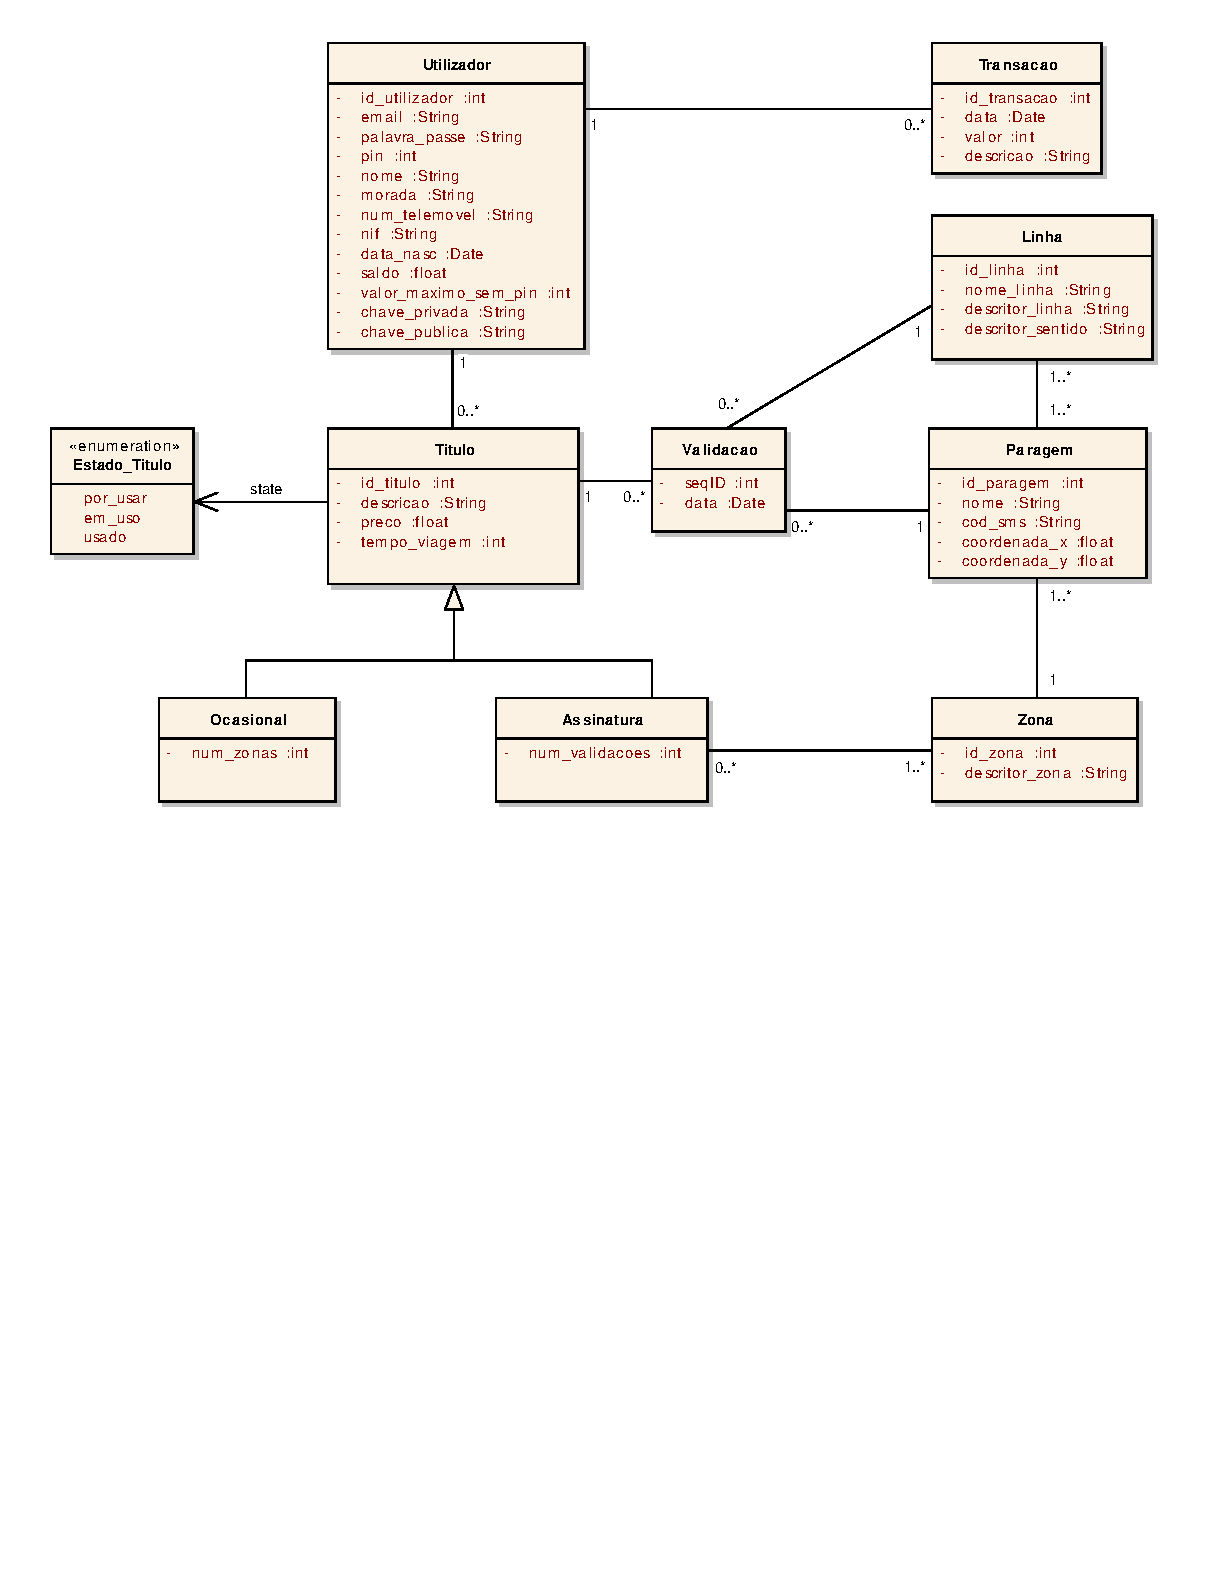
\includegraphics[scale=0.8]{class_diagram}
    \caption{Modelo Concetual}
    \label{fig:class_diagram}
  \end{center}
\end{figure}

\subsection{Utilizador}

Sendo uma aplicação de uso personalizado, é necessário associar toda a informação a um determinado utilizador. Para além dos dados pessoais do utilizador (nome, morada, número de telemóvel, Número de Informação Fiscal e data de nascimento), são também armazenados os dados de autenticação (endereço de correio eletrónico, palavra-passe e PIN numérico) e dados relacionados com a aplicação (saldo atual do utilizador e chaves de encriptação - pública e privada).
\\O elemento que garante a unicidade do utilizador é o endereço de correio eletrónico, pelo que após o registo, o utilizador não o poderá alterar. Por se tratar de um número único e invariável, também o Número de Identificação Fiscal não pode ser alterado através da aplicação, servindo para confirmação de identidade caso seja solicitado por parte do revisor.

\subsection{Título}

Os títulos são a componente central da aplicação, sendo que é através deles que se processam as principais funcionalidades da aplicação. Apesar de poder ser de diferentes tipos (Ocasional, Andante 24 e Assinatura Mensal), os diversos títulos possuem características em comum: descrição, preço e tempo de viagem. Para além disso, cada título tem associado a si um determinado estado (Por Usar, Em Uso ou Usado) e um conjunto de validações.

\subsubsection{Ocasional}

Em termos concetuais, o conceito ocasional engloba tanto os títulos ocasionais como os títulos Andante 24, por se basearem no mesmo princípio: uso limitado durante um determinado período de tempo e pelo número de zonas estipulado na tipologia do título. A única diferença prende-se com o facto de num título ocasional, o tempo de viagem ser calculado em função da tipologia e num título Andante 24, ser sempre de vinte e quatro horas.
\\Para além dos atributos herdados, é também necessário saber o número de zonas permitidas durante a utilização do título.

\subsubsection{Assinatura}

A assinatura é o modelo mensal, com número ilimitado de utilizações dentro do mês estipulado e nas zonas previamente selecionadas. Para além disso, a assinatura é de uso pessoal e intransmissível.
\\Para disponibilizar alguma informação extra ao utilizador, é também guardado o número de validações. Pode ser utilizado, no futuro, para aconselhar o utilizador a utilizar títulos ocasionais caso o número de validações seja baixo, por exemplo.

\subsection{Validação}
Uma validação é o conceito que relaciona a utilização de um determinado título a uma paragem e linha, registando a data e hora, e tendo associado um número sequencial único que serve para controlo por parte do revisor.

\subsection{Paragem}
Paragem é a localização física onde os veículos de determinadas linhas efetuam paragem, permitindo a entrada e saída de passageiros. Sendo uma das funcionalidades da aplicação, a apresentação das paragens mais próximas da localização do utilizador, é necessário saber as coordenadas de cada paragem, bem como a informação que a identifica unicamente.

\subsection{Linha}
Linha corresponde ao trajeto efetuado pelos veículos e que é constituído por diversas paragens. Para além de identificar unicamente cada linha, é necessário distinguir também o sentido do trajeto, pois, em muitos casos, o percurso efetuado (e respetivas paragens) difere no sentido de ida e de volta.

\subsection{Zona}
Partindo da designação de zona, do sistema Andante, é o conceito que permite ao utilizador identificar a tipologia do título a adquirir para determinada viagem. Cada paragem tem uma zona associada.

\subsection{Transação}
Uma transação é uma operação efetuada na aplicação que envolva movimentos monetários. Isto envolve tanto o carregamento da carteira virtual, como a compra de títulos. Este conceito é fundamental para permitir ao utilizador visualizar o histórico de operações efetuadas na aplicação.

\section{Arquitetura}

A aplicação baseia-se numa arquitetura Servidor-Cliente tradicional, com utilização de uma base de dados de suporte local, mas que serve apenas para acelerar alguns processos, sendo sempre necessário comunicar ao servidor quaisquer alterações que sejam feitas.
\\A aplicação comunica com o servidor através de ligação à Internet, utilizando serviços \web com API própria. Alguns dos serviços em utilização são os mesmos que se encontram na aplicação Move-Me pois fornecem informação pertinente para ambas as aplicações e também tendo em foco uma futura integração das duas. Ver Figura~\ref{fig:architecture}.

\begin{figure}[t]
  \begin{center}
    \leavevmode
    \includegraphics[scale=0.8]{architecture}
    \caption{Arquitetura Servidor-Cliente}
    \label{fig:architecture}
  \end{center}
\end{figure}

\section{Casos de Uso}

\subsection{Compra}

O primeiro passo a realizar, tal como acontece hoje em dia, é a compra de títulos de viagem. Esta compra pode ser feita de forma simples, selecionando a modalidade desejada, configurando-a (número de zonas e quantidade no caso dos títulos Ocasionais e Andante 24; escolha de zonas no caso da Assinatura) e finalizando a compra após confirmação dos detalhes.
\\Os preços utilizados são exatamente os mesmos em vigor nos postos de venda tradicionais e, tal como acontece atualmente, na compra de 10 títulos ocasionais ou Andante 24, é oferecido um título extra com a mesma tipologia.
\\Baseado no sistema Andante, a assinatura pode ser comprada desde o dia 16 do mês anterior até ao dia 15 do mês corrente. Como tal, caso o utilizador não compre a assinatura até ao dia 15, terá de viajar o resto do mês com títulos ocasionais. Apenas poderá comprar a assinatura para o mês seguinte, tal como acontece nos postos de venda tradicionais.
\\Para além de ser apresentado o saldo atual da carteira virtual, o utilizador consegue facilmente visualizar quais os títulos que tem disponíveis e saber assim se tem ou não necessidade de comprar um novo título.

\subsection{Validação}

Para poder viajar nos veículos de transportes públicos, o utilizador deve proceder à validação de um dos títulos disponíveis. Para tal deve, de antemão, garantir que possui o título necessário para a viagem que vai realizar.
\\Antes de realizar a validação do título é necessário selecionar a paragem e linha de entrada. A aplicação tenta, de forma automática, calcular a posição do utilizador e apresentar as paragens encontradas num raio de 80 metros, permitindo assim uma margem de erro de cálculo. No entanto, caso não seja possível calcular a posição atual do utilizador ou esta seja errada, é possível uma introdução manual da paragem, escolhendo o operador, a linha e finalmente a paragem.
\\Após a escolha da paragem, são listadas todas as linhas que param na paragem selecionada, permitindo ao utilizador escolher aquela onde vai entrar.
\\Concluído o processo de validação, o utilizador pode viajar normalmente no veículo e será criada uma notificação no telemóvel que lhe indica o tempo restante e o título em uso. Para além disso, essa notificação permite aceder ao menu de fiscalização, caso solicitado pelo revisor.

\subsection{Consulta}

É importante também aceder ao estado atual da carteira de títulos e da carteira virtual. Muitas vezes os utilizadores deparam-se com o problema de estarem em casa e não saberem se têm títulos carregados para poder efetuar uma viagem, tendo de se deslocarem a um posto de venda para efetuar essa verificação. Isso muitas vezes implica a perda do veículo desejado ou alterações no planeamento diário.
\\A aplicação permite ao utilizador consultar em qualquer altura quais os títulos que tem disponíveis, bem como as operações que efetuou (carregamentos, compras, etc.). Para além disso permite-lhe ainda visualizar o histórico de validações efetuadas, separando os títulos ocasionais da assinatura, porque normalmente existe uma discrepância no número de validações dum tipo e doutro sendo mais fácil a visualização em separado.

%\begin{lstlisting}[float,language=Java, label=src:mapreduce, caption=Example map and reduce functions for word counting]
%map(String key, String value): 
%// key: document name 
%// value: document contents 
%for each word w in value:
%EmitIntermediate(w, "1");
%
%reduce(String key, Iterator values):
%// key: a word 
%// values: a list of counts 
%int result = 0;
%for each v in values: 
%result += ParseInt(v);
%
%Emit(AsString(result))
%\end{lstlisting}


\section{Resumo ou Conclusões}